\documentclass[11pt, oneside, final]{article} 
\usepackage[utf8]{inputenc} 
\usepackage{a4wide} 
\usepackage[russian]{babel} 
\usepackage{graphicx} 
\usepackage{epstopdf} 
\usepackage{amsmath} 
\usepackage{amsfonts} 
\usepackage{amssymb} 
\usepackage{amsthm}
\usepackage{epstopdf}
\usepackage{float}
\usepackage{subcaption}
\usepackage[perpage]{footmisc}

%\newtheoremstyle{mytheorem}% name of the style to be used
%  {}% measure of space to leave above the theorem. E.g.: 3pt
%  {}% measure of space to leave below the theorem. E.g.: 3pt
%  {}% name of font to use in the body of the theorem
%  {}% measure of space to indent
%  {}% name of head font
%  {:}% punctuation between head and body
%  { }% space after theorem head; " " = normal interword spacewww
%  {}% Manually specify head
%\theoremstyle{mytheorem}
\newtheoremstyle{break}%
  {}{}%
  {\itshape}{}%
  {\bfseries}{}%  % Note that final punctuation is omitted.
  {\newline}{}
\theoremstyle{break}
\newtheorem*{PMP}{Принцип Максимума Понтрягина} 
\numberwithin{equation}{section} 
\theoremstyle{plain}
\newtheorem{theorem}{Теорема}[section] 
\newtheorem{property}{Свойство}[section] 
\newtheorem{corollary}{Следствие}[theorem] 
\newtheorem{lemma}[theorem]{Лемма} 
\newtheorem*{statement}{Утверждение} 
\theoremstyle{definition}
\newtheorem{definition}{Определение}[section] 
\renewenvironment{proof}{
\noindent\textit{Доказательство: }} {\qed}
\newcounter{icount}
\graphicspath{{figures/}}
%commands
\newcommand \bitem[1][]{
\item \textbf{#1}} 
\newcommand \four[1][\lambda]{\mathfrak{F}(#1)} 
\newcommand \fft[1][\lambda]{F(#1)} 
\newcommand \rarrow{\rightarrow} 
\newcommand \real{\mathbb{R}}
\newcommand \intinf[1][{\,dt}]{ \int\limits_{-\infty}^{+\infty}{{#1}}} 
\renewcommand \qed{$\blacksquare$}
\newcommand{\scalar}[2]{\langle #1, #2\,\rangle}
\DeclareMathOperator{\Argmax}{Argmax}

\DeclareMathOperator{\sgn}{sgn}
\DeclareMathOperator{\const}{const}

\begin{document}

%Title
    \thispagestyle{empty}
    \begin{center}
        \ \vspace{-3cm}
    
        
\includegraphics[width=0.5
        \textwidth]{msu}\\
        {\scshape Московский государственный университет имени М.~В.~Ломоносова}\\
        Факультет вычислительной математики и кибернетики\\
        Кафедра системного анализа
    
        \vfill
    
        {\LARGE Отчёт по практикуму}
    
        \vspace{1cm}
    
        {\Huge\bfseries "<Построение множества достижимости">} 
    \end{center}

    \vspace{1cm}
    \begin{flushright}
        \large \textit{Студент 315 группы}\\
        В.\,А.~Сливинский
    
        \vspace{5mm}
    
        \textit{Руководитель практикума}\\
        к.ф.-м.н., доцент П.\,А.~Точилин 
    \end{flushright}

    \vfill
    \begin{center}
        Москва, 2018 
    \end{center}
    \pagebreak

    %Contents
    \tableofcontents

    \pagebreak


    %Task

    \section{Постановка~задачи}
    \label{sec:task}
    \subsection{Формулировка~задачи} 
    \label{sub:general}
    Задано следующее обыкновенное дифференциальное уравнение:
    \begin{equation} 
        \label{eq:system:init} 
        \ddot x + x \dot x - \arctg(x^2) + x^2\cos(x^2) = u
    \end{equation}
    Здесь, \(x \in \real,\, u \in \real \). Кроме того, на управление \( u \) наложено дополнительное ограничение \(u \in \mathfrak{U}, \: \mathfrak{U} = \left[-\alpha, \alpha\right], \: \alpha > 0 \). Задан начальный момент времени \(t_0 = 0\) и начальная позиция \(x(t_0) = \dot x(t_0) = 0\). Необходимо построить множество достижимости \(\mathcal{X}(t, t_0, x(t_0), \dot x(t_0))\) (множество пар \((x(t), \dot x(t))\)) в классе программных управлений в заданный момент времени \(t \geqslant t_0\). 
    Требуется: 
    \begin{enumerate} 
        \item Написать в среде Matlab функцию \texttt{reachset(alpha, t)}, которая по заданным значениям параметров \(\alpha > 0, \: t \geqslant t_0\) рассчитывает приближенно множество достижимости \(\mathcal{X}(t, t_0, x(t_0), \dot x(t_0))\). На выходе функции~--- два массива \texttt{X, Y} с упорядоченными координатами точек многоугольника, аппроксимирующего границу множества достижимости. Точки в этих массивах должны быть упорядочены так, чтобы их без дополнительной обработки можно было подавать на фход функции \texttt{plot}. Также, функция должна предусматривать режим работы, в котором, помимо границы множества достижимости, возвращаются также координаты линии переключения оптимального управления;
        \item Реализовать функцию \texttt{reachsetdyn(alpha, t1, t2, N, filename)}, которая, используя функцию \texttt{reachset}, строит множества достижимости для моментов времени \(\tau_i = t_1 + \frac{(t_2 - t_1)\cdot i}{N}\). Здесь, \(t_2 \geqslant t_1 \geqslant t_0,\, N\)~--- натуральное число. Для каждого момента времени \(\tau_i\) функция должна отобразить многоугольник, аппроксимирующий границу множества достижимости. Результат работы функции должен быть сохранён в виде видеофайла \texttt{filename.avi}. Необходимо также предусмотреть вариант работы функции (при отсутствии параметра \texttt{filename}) без сохранения в файл, с выводом непосредственно на экран. Как частный случай, при \(t_2 = t_1\) функция должна строить границу множества достижимости в один фиксированный момент времени.
    \end{enumerate}
    \pagebreak
    %Formal task
    \subsection{Формализация~задачи} 
    \label{sub:formal}
    Прежде всего, нормализуем систему~\eqref{eq:system:init}:
    \begin{equation}
        \label{eq:system}
        \left\{
        \begin{aligned}
            &\dot x_1 = x_2 \\
            &\dot x_2 = u - x_1^2 \cos(x_1^2) + \arctg(x_1^2) - x_1\cdot x_2\\
        \end{aligned}
        \right.
    \end{equation}   
    Здесь, \(x_1 = x,\: x_2 = \dot x\). Управление \(u\) будем полагать \emph{кусочно--непрерывной} функцией.
    \begin{definition} Для любого времени \(t \geqslant t_0\) множество 
        \begin{multline*}
            \mathcal{X}[t] = \mathcal{X}(t, t_0, x_1(t_0), x_2(t_0)) =\\ = \Bigg\{(x_1(t), x_2(t)) \in \real^2:\; \exists u^* = u^*(t):\: |u*(\tau)| \leqslant \alpha \; \dot \forall \tau \in [t_0, t],\\\left.\: (x_1(t), x_2(t)) = (x_1(t, t_0, x_1(t_0), x_2(t_0)), x_2(t, t_0, x_1(t_0), x_2(t_0)))\bigg\rvert_{u^*(t)}\right\}
        \end{multline*}
        будем называть \emph{множеством достижимости для системы~\eqref{eq:system} в момент времени \(t \geqslant t_0\)}.
    \end{definition}
    \pagebreak
    \section{Некоторые~необходимые~теоретические~выкладки}
    \label{sec:theory}
    Для начала, выпишем для задачи~\eqref{eq:system} функцию Гамильтона--Понтрягина:
    \begin{equation*}       \mathcal{H}(\psi,x,u)=\left<\psi,f(x,u)\right>=\psi_1x_2+\psi_2\left(u - x_1^2 \cos(x_1^2) + \arctg(x_1^2) - x_1\cdot x_2\right)
    \end{equation*}
    Введём вспомогательную функцию
    \[
    \mathcal{M}(\psi,x)=\sup\limits_{u\in[-\alpha,\alpha]}\mathcal{H}(\psi,x,u).
    \]
    Теперь, сформулируем принцип максимума Понтрягина для задачи достижимости
    \begin{PMP}[в формулировке из \cite{Roublev:optimal}]
    	Пусть \( \left(x^*(\cdot),u^*(\cdot)\right) \)~---~оптимальная по быстродействию пара для задачи~\eqref{eq:system} при \( t_1=t_1^* \) (здесь \( t\in[0,t_1^*] \)). Тогда существует функция \( \psi^*(\cdot):[0,t_1^*]\rightarrow\mathbb{R}^2 \) такая, что:
    \begin{align}
            & \psi^* \not \equiv0 \label{eq:nontriv} \\
            & \dot{\psi}^*(t)=-\dfrac{\partial \mathcal{H}}{\partial x}\bigg|_{\substack{ \psi=\psi^*(t)\\ x=x^*(t) \\ u=u^*(t)}}  \label{eq:conj} \\
            & u^*(t) \in \Argmax\limits_{u\in[-\alpha,\alpha]} \mathcal{H}(\psi^*(t),x^*(t),u) \; \dot \forall t\in[0,t_1^*] \label{eq:max} \\
            & \mathcal{M}(\psi^*(t),x^*(t))\equiv\const\geqslant 0
        \end{align}
        
    \end{PMP}
    \noindent
    Доказательство данной теоремы в общем случае приведено, например, в~\cite{Pontr'yaginEtAl:maximum}. Систему \eqref{eq:conj} называют \emph{сопряжённой системой}, условие~\eqref{eq:max}~--- условием максимума, а условие~\eqref{eq:nontriv}~--- условием нетривиальности (из него следует, что \( \psi^*(t)\ne0 \) для всех \( t\in[0,t_1^*] \)). Условие~\eqref{eq:max} позволит в явном виде выписать оптимальное управление. \\ Сформулируем также \textit{теорему о нулях \( \psi_2 \) и \( x_2 \)}\footnote{Её доказательство  приведено в \cite{Roublev:optimal}}:

\begin{theorem} \label{thm:zeros}
	Пусть \( \tau_1<\tau_2 \) и
	\begin{enumerate}
		\item \( \psi_2(\tau_1)=\psi_2(\tau_2)=0 \) и \( x_2(\tau_1)=0 \) \( \Rightarrow x_2(\tau_2)=0 \);
		
		\item \( x_2(\tau_1)=x_2(\tau_2)=0 \), \( x_2(t)\ne0 \) при \( t\in(\tau_1,\tau_2) \) и \( \psi_2(\tau_1)=0 \) \( \Rightarrow\psi_2(\tau_2)=0 \).
		
		\item \( \psi_2(\tau_1)=\psi_2(\tau_2)=0 \) и \( x_2(\tau_1)\ne0 \) \( \Rightarrow x_2(\tau_2)\ne0 \), но \( \exists t'\in(\tau_1,\tau_2):x_2(t')=0 \).
		
		\item \( x_2(\tau_1)=x_2(\tau_2)=0 \), \( x_2(t)\ne0 \) при \( t\in(\tau_1,\tau_2) \) и \( \psi_2(\tau_1)\ne0 \) \( \Rightarrow\psi_2(\tau_2)\ne0 \), но \( \exists t''\in(\tau_1,\tau_2):\psi_2(t'')=0 \).
	\end{enumerate}
\end{theorem}
Обратим внимание, что функция \( \psi_2(\cdot) \) имеет не более чем конечное число нулей на отрезке \( [0,t_1^*] \) (в противном случае, получим противоречие с \eqref{eq:nontriv}).
    \section{Описание алгоритма}
    \label{subs:conj} 
    Для начала, выпишем сопряженную систему:
    \begin{equation}
        \label{eq:sys:conj}
        \left\{
        \begin{aligned}
            & \dot \psi_1 = \psi_2\cdot\left(x_2 + 2 x_1\cos(x_1^2) + 2 x_1^3\sin(x_1^2) - \dfrac{4x_1\arctg(x_1)}{x_1^4 + 1}\right)\\
            & \dot \psi_2 = \psi_2 x_1 - \psi_1\\
        \end{aligned}
        \right.
    \end{equation}
    Из~\eqref{eq:max} получим:
    \[
    u^*(t)=\begin{cases}
    \alpha,&\psi_2(t)>0,\\
    [-\alpha,\alpha],&\psi_2(t)=0,\\
    -\alpha,&\psi_2(t)<0.
    \end{cases}
    \]
    Обратим внимание, что особого режима не возникает, так как в противном случае получаем нулевой вектор \( \psi \), что противоречит~\eqref{eq:nontriv}.
    Дополнительно, обозначим за \(S_+\) систему~\eqref{eq:system} при \(u = \alpha\), а за \(S_-\) систему~\eqref{eq:system} при \(u = -\alpha\). Стало быть, в силу теоремы (\ref{thm:zeros}), для решения задачи применим следующий алгоритм:
    \begin{itemize}
    	\item Решаем систему \( S_+ \) из начальной (нулевой) точки до момента \( t_+:\; x_2(t_+) = 0 \);
    	\item Строим разбиение отрезка \( [0,t_+] \). Обозначим точку этого разбиения через \( t^i_+ \);
    	\item Решаем систему \( S_- \), присоединив к ней сопряжённую систему~\eqref{eq:sys:conj}, с начальными условиями \( (x_1(t^i_+),x_2(t^i_+),1,0) \) (в силу инвариантности решения системы~\eqref{eq:sys:conj}) относительно умножения на положительную константу и в силу того, что \( \psi_1(t_+)>0 \), можно нормировать \( \psi_1(t_+)=1 \)) до момента \( \psi_2(\hat{t}^i_+) \) (из теоремы~\eqref{thm:zeros} следует, что такой момент найдётся);
    	\item Далее решаем систему \( S_+ \) и присоединённую к ней сопряжённую систему~\eqref{eq:sys:conj} с начальными условиями \( (x_1(\hat{t}^i_+),x_2(\hat{t}^i_+),-1,0) \) до следующего переключения. Повторяем последние два пункта до момента \( t \), заданного пользователем;
    	\item Аналогичные действия проводим для системы \( S_- \);
    	\item Соединяем концы полученных траекторий;
	    \item Исследуем отрезки полученной ломаной. Если расстояние между каким-то соседними точками больше некоторого фиксированного значения (параметра функции), то производится дополнительное подразбиение отрезка \( [t_{i},t_{i+1}] \), где \( t_{i} \) и \( t_{i+1} \)~---~моменты первого переключения для этих точек. Для этого подразбиения рассчитываются новые траектории, концы которых включаются в новую аппроксимацию. Повторяем эти действия, пока каждая сторона многоугольника не станет меньше или равна этого заданного значения. Таким образом, будет получена кривая соответствующей гладкости и устранена (с некоторой точностью, зависящей от заданного значения) ошибка попадания неподвижных точек системы внуть множества достижимости;
    	\item Удаляем самопересечения. Пройдём по точкам полученной ломаной, запоминая моменты пересечения отрезков. Затем, удалим участки, заключенные между точками пересечений, если до них было чётное (или ноль) число пересечений; это позволяет устранить "<петли">.
    \end{itemize}
    Отметим, что, во--первых, для вывода кривой переключений достаточно лишь запоминать моменты переключения при решении соответствующих систем, а, во--вторых, поскольку одна из фазовых переменных в системе при достаточно больших значениях \(t\) и \(\alpha\) очень быстро растёт, дополнительно будем "<обрезать"> траектории, выходящие за некоторый радиус (параметр функции). Помимо этого, в функции также ищутся стационарные точки систем \(S_+\) и \(S_-\): для этого, поскольку в них \(x_2 = 0\), достаточно при помощи функции \texttt{fzero} отыскать нули функций \(\arctg(x_1^2)  - x_1^2\cos(x_1^2) \pm \alpha\) с начальными приближениями из равномерной сетки \([x_{min}, x_{max}]\), где \(x_{min} = \min\limits_{\mathtt{X}}x_1,\; x_{max} = \max\limits_{\mathtt{X}}x_1\).\footnote{\texttt{X}~--- вектор, возвращаемый функцией \texttt{reachset}, состоящий из абсцисс границы множества достижимости} 
    \pagebreak
    \section{Примеры работы программы}
    \label{sec:examples}
    \begin{figure}[!htpb]
            \centering
            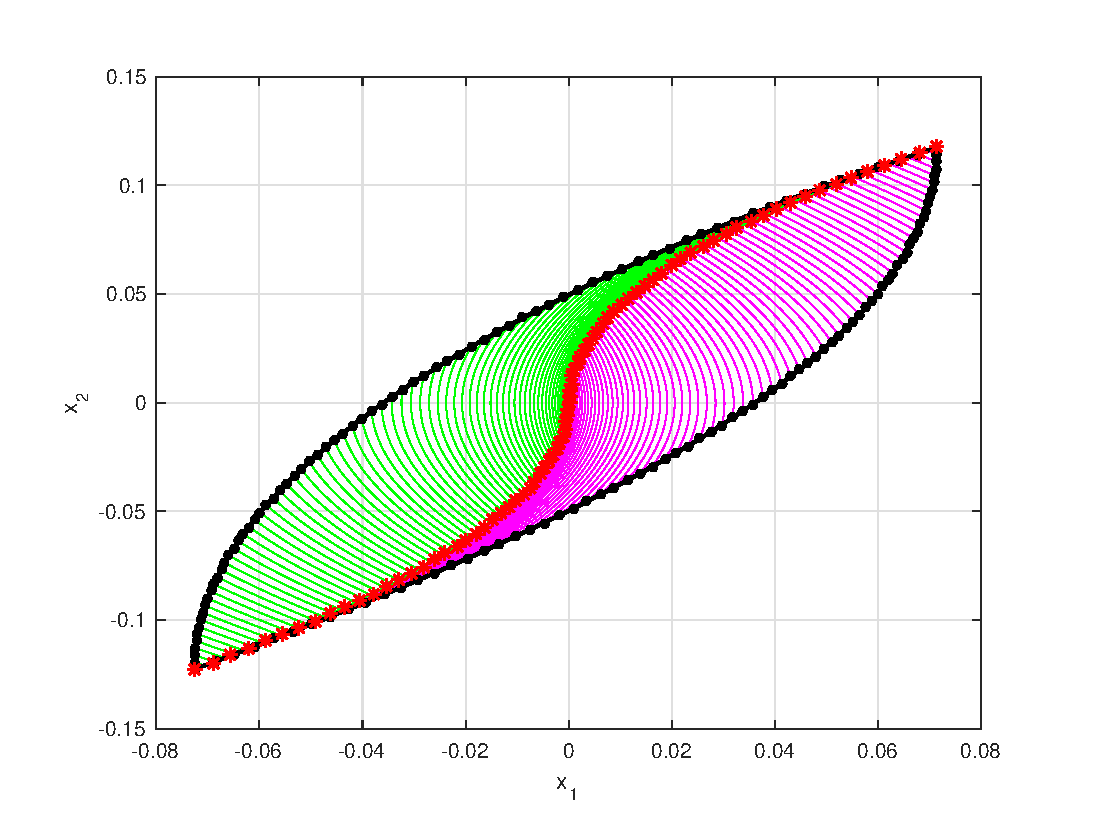
\includegraphics[width=\linewidth]{figa01t12}
            \label{pic:1}
            \caption{Множество достижимости при \(\alpha = 0.1,\: t = 1.2\), с трассировкой траекторий, красным отмечена кривая переключений, чёрным~--- граница множества достижимости}
    \end{figure}
    \begin{figure}[!htpb]
            \centering
            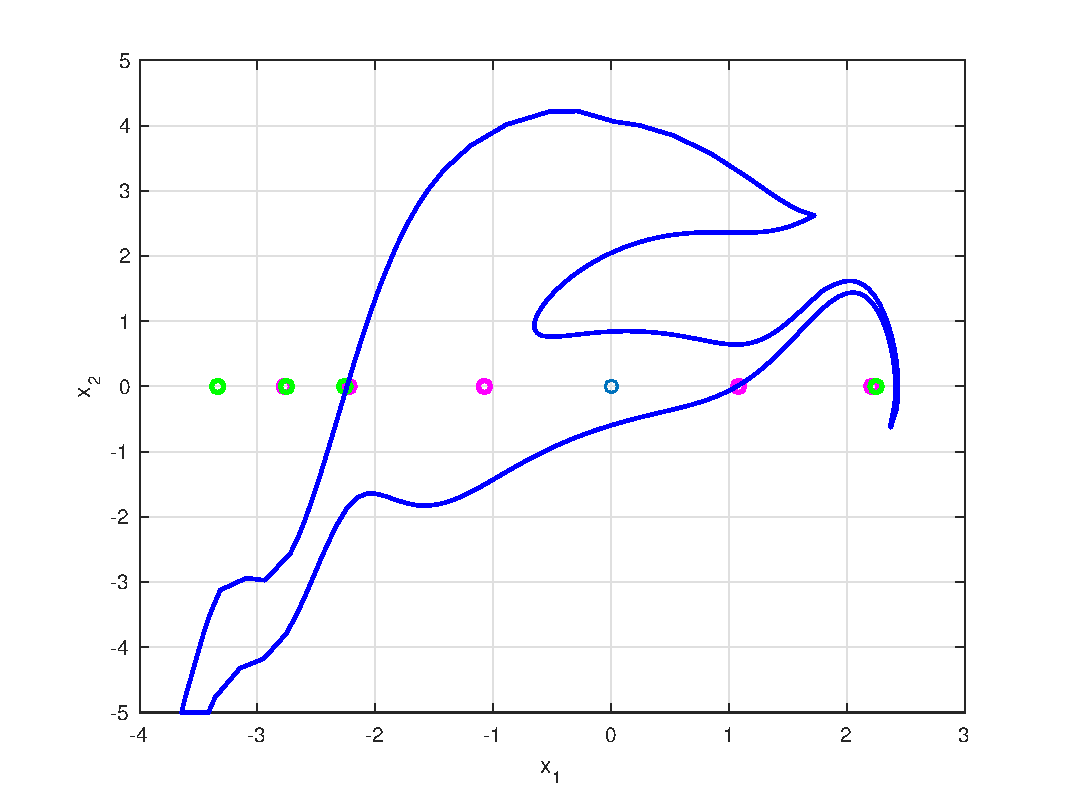
\includegraphics[width=\linewidth]{figa05t45}
            \label{pic:2}
            \caption{Множество достижимости при \(\alpha = 0.4,\: t = 4.25\), синим отмечена граница множества достижимости, дополнительно отмечены стационарные точки систем \(S_+\) и \(S_-\); здесь установлен сравнительно небольшой радиус ограничения траекторий \texttt{maxRadius} = 5}
    \end{figure}
    \begin{figure}[!htpb]
            \centering
            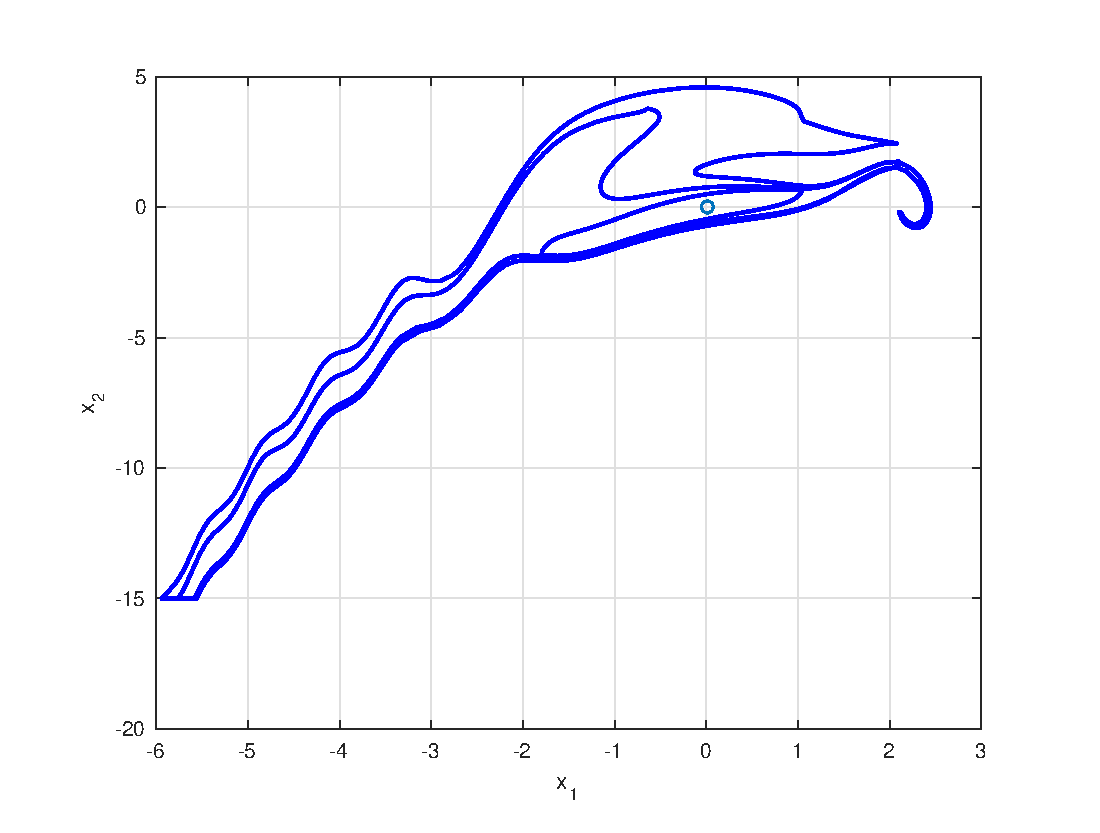
\includegraphics[width=\linewidth]{figa05t1545}
            \label{pic:3}
            \caption{Эволюция множества достижимости при \(\alpha = 0.5,\: t = 1.5\dots4.5\), синим отмечена граница множества достижимости}
    \end{figure}
    \pagebreak
    \begin{thebibliography}{0}
        \addcontentsline{toc}{section}{Список литературы}
        \bibitem{Roublev:optimal} И. В.~Рублёв. \emph{Лекционный курс Оптимальное Управление (Нелинейные Системы)},
        кафедра Системного~Анализа, Факультет Вычислительной Математики и Кибернетики, МГУ~им.~М.~В.~Ломоносова, 
        2018
        \bibitem{RoublevTochilin:matlab} Точилин~П.~А. \emph{Лекционный курс Программирование на языке \texttt{MATLAB}},
        кафедра Системного~Анализа, Факультет Вычислительной Математики и Кибернетики, МГУ~им.~М.~В.~Ломоносова, 
        2017~-- 2018
        \bibitem{Pontr'yaginEtAl:maximum} Понтрягин Л. С., Болтянский В. Г., Гамкрелидзе Р. В., Мищенко Е. Ф.~\emph{Математическая~теория~оптимальных~процессов}, — М.: Наука, 1976.
        \bibitem{Matlab:help} Справочные средства языка \texttt{MATLAB}
    \end{thebibliography}
\end{document}
